\title{Introductory Electricity, Magnetism, and Optics Practice Problems}
\author{Cyrus Vandrevala}

\documentclass[11pt]{article}
\usepackage{amsmath}
\usepackage[margin=2.5cm]{geometry}
\usepackage[pdftex]{graphicx}

\begin{document}

\maketitle
\tableofcontents
\vspace{50pt}

\subsection*{Useful Constants}
Electron Mass = $9.11 \times 10^{-31}$ kg \\*
Proton Mass = $1.67 \times 10^{-27}$ kg \\*
Elementary Charge = $1.602 \times 10^{-19}$ C \\*
Coulomb's Constant = $8.99 \times 10^9$ Nm$^2$/C$^2$ \\*
Gravitational Constant = $6.67 \times 10^{-11}$ m$^3$/kg$\cdot s^2$ \\*
Avogadro's Number = $ 6.02 \times 10^{23}$ atoms/mole \\*\\*
Atomic Number of Uranium = 92 \\*
Atomic Number of Copper = 29 \\*
Molar Mass of Copper = 63.5 g/mole \\*
Mass of the Earth = $5.97 \times 10^{24}$ kg\\*
Mass of the Moon = $7.35 \times 10^{22}$ kg

%%%%%%%%%%%%%%%%%%%%%%%%%%%%%%%%%%%%%%%%%%%%%%%%%%%%%%%%%%%%%%%%%%%%%%%%%%%%%%

\pagebreak
\section{Quantized Electric Charge and Charging Objects}
\vspace{10pt}

\subsection{Electric Charge Units}
What is the basic unit of electric charge?\\* \\*
$\Rightarrow$ Coulomb

\subsection{Transfer of Electrons}
I rub a piece of silk against a glass rod in order to charge up the rod.  If the final charge on the rod is +2.3 $\mu$C, how many electrons were transferred from the rod to the silk? \\* \\*
$\Rightarrow 1.4 \times 10^{13}$ electrons

\subsection{Charge Within a Uranium Nucleus}
What is the net charge within the nucleus of an atom of U-238? \\* \\*
$\Rightarrow 1.5 \times 10^{-17}$ C

\subsection{Number of Electrons in Copper}
Estimate the number of electrons in a 1.0 kg block of copper that has been charged to +10 $\mu$C. \\* \\*
$\Rightarrow 2.7 \times 10^{26}$ electrons

\subsection{Charging an Object \#1}
I bring a charged insulator close to an uncharged conductor (not touching).  I then ground the conductor.  This method of charging the conductor is called charging by \underline{\hspace{1cm}}. \\* \\*
$\Rightarrow$ Induction

\subsection{Charging an Object \#2}
I touch an uncharged conductor to a second negatively charged conductor.  This method of charging an object is called charging by \underline{\hspace{1cm}}. \\* \\*
$\Rightarrow$ Contact

\subsection{Charging an Object \#3}
I rub a glass rod against a silk cloth in order to charge up the glass rod.  This is an example of charging by \underline{\hspace{1cm}}. \\* \\*
$\Rightarrow$ Friction

%%%%%%%%%%%%%%%%%%%%%%%%%%%%%%%%%%%%%%%%%%%%%%%%%%%%%%%%%%%%%%%%%%%%%%%%%%%%%%

\pagebreak
\section{Coulomb's Force Law}
\vspace{10pt}

\subsection{Hydrogen Atom}
In a hydrogen atom, a proton is separated from an electron by an average distance of about $5.3 \times 10^{-11}$ meters.  Calculate the electrostatic force of attraction by the proton on the electron.  Do the same for the electron on the proton. \\* \\*
$\Rightarrow 8.2 \times 10^{-8}$ N, Same For Both

\subsection{Force at the Center of a Square}
Suppose I place four charges (each +Q) at the four vertices of a square with side length L.  What is the magnitude of the net force on a positive point charge (+q) located at the center of the square? \\* \\*
$\Rightarrow$ 0 N

\subsection{Equilibrium Point}
Suppose I place a charge of $Q_1$ = +1.0 nC at the point (1 m, 0 m) and a charge of $Q_2$ = -2.5 nC at the point (0 m, 0 m).  At what point in the xy-plane could I put a negative charge of $Q_3$ = -5.0 $\mu$C such that $Q_3$ would feel no net electrostatic force? \\* \\*
$\Rightarrow$ (2.7 m, 0 m)

\subsection{Electrical vs. Gravitational Force}
Suppose the moon were held in orbit due to an electrical force instead of a gravitational force.  Assume that the Earth and the moon have equal charge magnitudes with opposite sign (i.e. $Q_{Earth}$ = +q and $Q_{Moon}$ = -q).  How large would these charges have to be in order to maintain the current stable orbit? \\* \\*
$\Rightarrow |Q_{Earth}| = |Q_{Moon}| = 5.71\times10^{13}$ C

\pagebreak
\subsection{Charged Pendulum}
Consider the double pendulum setup shown below.  Two small spherical bobs, each with mass M hang from strings of length L.  After a short time, the bobs reach the equilibrium position as shown where the angle $\theta$ is measured from the vertical.  Derive an expression for the charge on each bob.\\* \\*
$\Rightarrow Q = \sqrt{\frac{mgL^2sin^3\theta}{kcos\theta}}$ \\*

\begin{center}
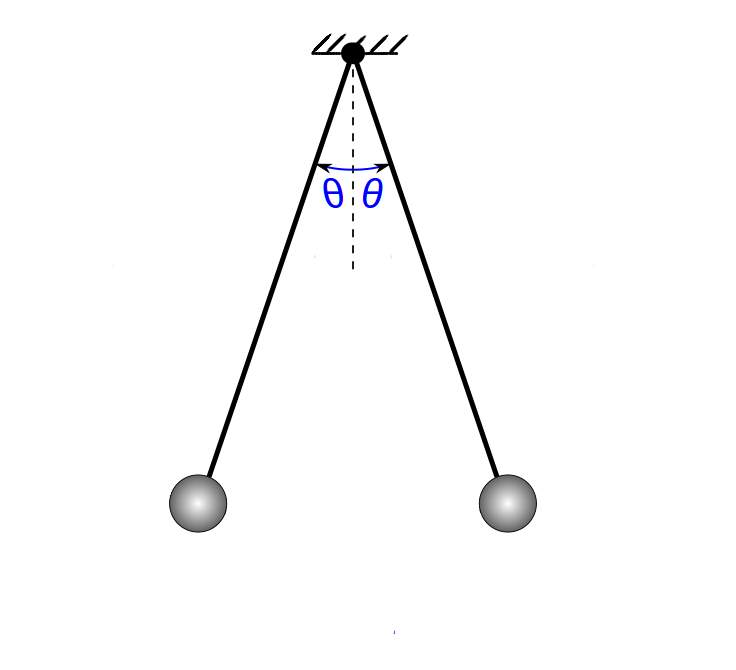
\includegraphics[scale=0.25]{Images/pendulum.png}
\end{center}

%%%%%%%%%%%%%%%%%%%%%%%%%%%%%%%%%%%%%%%%%%%%%%%%%%%%%%%%%%%%%%%%%%%%%%%%%%%%%%

\pagebreak
\section{Continuous Electric Charge}
\vspace{10pt}

\subsection{Charge at the Center of a Ring}
Consider a charged ring in the xy-plane, centered at the origin, with charge density $\rho$ = cos($\theta$) where $\theta$ is the angle about the ring in standard orientation.  If I place a positive charge at the center of the ring, which way will it move? \\* \\*
$\Rightarrow -\hat{x}$ direction

\subsection{Uniformly Charged Ring}
Calculate the electric field along the axis of a uniformly charged ring (radius R, net charge Q). \\* \\*
$\Rightarrow \vec{E} = \frac{kQz}{(z^2 + R^2)^{3/2}}\hat{z}$

\subsection{Uniformly Charged Ring (Difficult - Extra Credit)}
Show that for small distances, the electric field around the center of the uniformly charged ring is linear with distance.  Then, show that a particle released near the center of the ring experiences simple harmonic motion. \\* \\*
\begin{equation}
\vec{E} = \frac{kQz}{(z^2 + R^2)^{3/2}}\hat{z} \approx \frac{kQz}{R^3}\hat{z}
\end{equation}

\begin{equation}
\vec{F} = m \vec{a}
\end{equation}
\begin{equation}
-\frac{kQz}{R^3} = m\frac{d^2z}{dt^2}
\end{equation}
\begin{equation}
\frac{d^2z}{dt^2} + \frac{kQz}{mR^3} = 0
\end{equation}
\begin{equation}
z(t) = Asin(\omega t)
\end{equation}
where
\begin{equation}
\omega = \sqrt{\frac{kQ}{mR^3}}
\end{equation}

\pagebreak
\subsection{Charged Line \#1}
A uniform line of charge extends from the point (0,0) to (1,0).  It has a net charge of +Q.  What is the electric field at the point (2,0)? \\* \\*
$\Rightarrow \frac{1}{2}kQ$

\subsection{Charged Line \#2 (Difficult)}
A uniform line of charge extends from the point (0,0) to (1,0).  It has a net charge of +Q.  What is the electric field at the point (2,1)?  Hint: You might need to consult a table of integrals for this problem. \\* \\*
$\Rightarrow \vec{E} = \frac{kQ}{\sqrt{10}}(\sqrt{5} - \sqrt{2})\hat{x} + \frac{kQ}{\sqrt{10}}(2\sqrt{2} - \sqrt{5})\hat{y}$

%%%%%%%%%%%%%%%%%%%%%%%%%%%%%%%%%%%%%%%%%%%%%%%%%%%%%%%%%%%%%%%%%%%%%%%%%%%%%%

\pagebreak
\section{Electric Field}
\vspace{10pt}

\subsection{Electron in an Electric Field \#1}
An electron is fired into a uniform electric field.  The initial velocity of the electron is given by $\vec{v} = 500 \hat{x} + 100 \hat{y} - 300 \hat{z}$, and the electric field is given by $\vec{E} = 100 \hat{x} + 200 \hat{y} - 150 \hat{z}$.  Calculate the magnitude of the acceleration of the electron at time t = 5 s. \\* \\*
$\Rightarrow |\vec{a}| = 4.735 \times 10^{13}$ m/s$^2$

\subsection{Electron in an Electric Field \#2}
An electron is fired into a region of uniform electric field given by $\vec{E} = 0.10\hat{y}$ N/C. At time t = 0 s, it is located at the origin with an initial velocity of $\vec{v_o} = 5.0 \times 10^5 \hat{x} + 3 \times 10^5 \hat{y}$  m/s.  What is the velocity of the particle at time t = 1.0 $\mu$s? \\* \\*
$\Rightarrow \vec{v} = (3.0\times10^5)\hat{x} + (2.8\times10^5)\hat{y}$ m/s

\subsection{Electron in an Electric Field \#3}
An electron is fired into a region of uniform electric field given by $\vec{E} = 10\hat{y}$. At time t = 0 s, it is located at the origin with an initial velocity of $\vec{v_o} = 5.0 \times 10^5 \hat{x} + 3 \times 10^5 \hat{y}$ m/s.  At what time during its trajectory does it intersect the x-axis again? \\* \\*
$\Rightarrow$ t = 341.6 ns

\subsection{Multiple Choice}
Which of the following statements is NOT true?

\begin{itemize}
	\item[A)] Electric field lines emanate from positive charges and terminate on negative charges.
	\item[B)] Electric field lines that are closely spaced imply a strong electric field.
	\item[C)] Positive point charges feel an electric force parallel to electric field lines.
	\item[D)] A positive point charge does not produce an electric field.
	\item[E)] There is a non-zero electric field at every finite distance around an electric dipole.
\end{itemize}
$\Rightarrow$ D

\pagebreak
\subsection{Pendulum in an Electric Field}
Consider a simple pendulum that has a bob with mass M and charge +Q as shown below.  The string of the pendulum has a length L.  A uniform electric field of magnitude E keeps the pendulum bob at equilibrium.  Derive an expression for $\theta$. \\* \\*
$\Rightarrow \theta = tan^{-1}(\frac{qE}{mg})$

\begin{center}
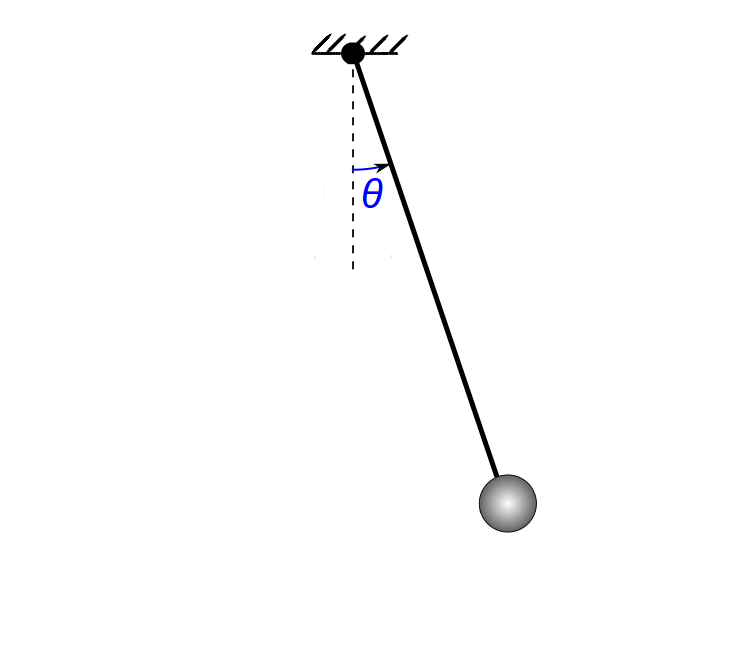
\includegraphics[scale=0.25]{Images/pendulum-efield.png}
\end{center}

%%%%%%%%%%%%%%%%%%%%%%%%%%%%%%%%%%%%%%%%%%%%%%%%%%%%%%%%%%%%%%%%%%%%%%%%%%%%%%

\pagebreak
\section{Electric Dipoles}
\vspace{10pt}

\subsection{Electric Field Due to a Dipole}
Consider an electric dipole with charges +Q and -Q located at x = +1 m and x = -1 m respectively.  Calculate the net electric field due to the dipole at x = 0 m. \\* \\*
$\Rightarrow -2kQ$ N/C $\hat{x}$

\subsection{Potential Energy of an Electric Dipole}
I place a dipole with dipole moment p = 10$\hat{z}$ C$\cdot$m in an electric field E = -100$\hat{x}$ N/C.  What is the potential energy of the dipole? \\* \\*
$\Rightarrow$ 0 J

\subsection{Maximum Potential Energy of an Electric Dipole}
Suppose I put an object with dipole moment 2.00 C$\cdot$m in a uniform electric field of magnitude 300 N/C.  What is the maximum possible value for the potential energy of the system? \\* \\*
$\Rightarrow$ 600 J

\subsection{Multiple Choice}
Which of the following statements is NOT true?

\begin{itemize}
	\item[A)] If a perfect electric dipole is placed into a uniform electric field, it can experience a net force.
	\item[B)] A perfect electric dipole consists of two equal and opposite point charges separated by a small distance.
	\item[C)] If a perfect electric dipole is placed into a non-uniform electric field, the dipole can experience a net force.
	\item[D)] If a perfect electric dipole is placed into a uniform electric field, the dipole can experience a net torque.
	\item[E)] If a perfect electric dipole is placed into a non-uniform electric field, the dipole can experience a net force.
\end{itemize}
$\Rightarrow$ A

\pagebreak
\subsection{Electric Dipole in an Electric Field}
I place an electric dipole in a uniform electric field as shown below.  What is the net force on the dipole?  What is the net torque on the dipole?  What is the electric potential energy of the dipole?

\begin{center}
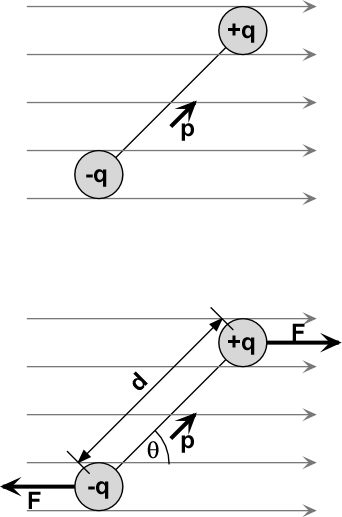
\includegraphics[scale=0.25]{Images/electric_dipole.png}
\end{center}

$\Rightarrow \vec{F} = 0$, \hspace{2mm}$\tau = dFsin\theta = dqEsin\theta$, \hspace{2mm}$U_E = -pEcos\theta$

%%%%%%%%%%%%%%%%%%%%%%%%%%%%%%%%%%%%%%%%%%%%%%%%%%%%%%%%%%%%%%%%%%%%%%%%%%%%%%

\pagebreak
\section{Electric Flux}

\subsection{Charge Density}
Charge per unit volume is defined as \underline{\hspace{1cm}}. \\* \\*
$\Rightarrow$ Charge Density

\subsection{Flux Through a Sphere}
Some region of space contains a uniform electric field given by $\vec{E} = 3\hat{i} + 4\hat{j}$ N/C.  I place a metal spherical shell of radius R = 1 m into the electric field.  What is the net electric flux through the sphere? \\* \\*
$\Rightarrow 0$ Nm$^2/C$

\subsection{Flux Around an Electric Dipole \#1}
An electric dipole is formed by two point charges (+Q and -Q) located at (1 m, 0 m) and (-1 m, 0 m) respectively.  I draw a closed elliptical surface such that the charges +Q and -Q are both located outside the ellipse.  What is the net electric flux through the ellipse? \\* \\*
$\Rightarrow 0$ Nm$^2/C$

\subsection{Flux Around an Electric Dipole \#2}
An electric dipole is formed by two point charges (+Q and -Q) located at (1 m, 0 m) and (-1 m, 0 m) respectively.  I draw a closed elliptical surface such that the charges +Q and -Q are both located inside the ellipse.  What is the net electric flux through the ellipse? \\* \\*
$\Rightarrow 0$ Nm$^2/C$

%%%%%%%%%%%%%%%%%%%%%%%%%%%%%%%%%%%%%%%%%%%%%%%%%%%%%%%%%%%%%%%%%%%%%%%%%%%%%%

\end{document}




